\appendix
\chapter{Réglage sur votre ToM+ (Twizy-cfg)}
\label{apx:tuning}

\section{Qu'est-ce que Twizy-cfg ?}

\href{http://github.com/dexterbg/Twizy-Cfg}{Twizy-Cfg} est un shell de configuration \textbf{open-source} et léger conçu pour le contrôleur de moteur SEVCON
Gen4 intégré dans la Renault Twizy, développé par \href{https://github.com/dexterbg}{dexterbg}. 
Développé pour fonctionner sur des microcontrôleurs Arduino équipés d'un module CAN-bus SPI MCP2515,
cet outil fournit aux hackers matériels, techniciens et passionnés de VE une interface en ligne
de commande directe pour interagir avec le système de transmission du véhicule via le port de
\textbf{diagnostic OBD-II} standard.\\

À son cœur, Twizy-Cfg agit comme un pont entre des commandes macro de \textit{haut niveau} et des opérations de
registre SDO (Service Data Object) CANopen de \textit{bas niveau}. Il permet un réglage et une
surveillance précis du groupe motopropulseur, offrant des fonctionnalités telles que :\\

\begin{itemize}
    \item Personnalisation du profil de conduite : Ajustement des paramètres clés de performance, notamment la puissance maximale, les limites de couple, la vitesse maximale et les rampes d'accélération.
    \item Gestion de l'énergie : Réglage fin des niveaux de récupération d'énergie pendant la roue libre et le freinage pour équilibrer l'autonomie de conduite et la force de freinage.
    \item Gestion des profils : Sauvegarde, chargement et restauration de profils de performance personnalisés directement depuis et vers l'EEPROM de l'Arduino.
    \item Diagnostics et accès bas niveau : Émission de commandes CANopen brutes et de requêtes de diagnostic OBD-II de base pour inspecter les états du contrôleur et les révisions du micrologiciel.  
\end{itemize}
\  \\
Cet appendice couvrira la façon dont ToM+ peut gérer une partition spéciale avec le logiciel
mentionné ci-dessus, adapté pour fonctionner sur sa carte ESP32 (puce ToM+).


\section{Prérequis avant de commencer}

\textbf{AVERTISSEMENT !} L'objectif de cet appendice est d'installer et de faire fonctionner dans la
boîte noire un micrologiciel alternatif, non codé par moi, en utilisant le matériel pour un
usage différent de celui pour lequel il a été conçu.
En suivant ce guide, vous aurez une \textbf{boîte noire à double démarrage}, avec le micrologiciel ToM+ et le
micrologiciel Twizy-cfg coexistant, chacun amorçable selon vos besoins.\\

Pour atteindre cet objectif, vous aurez besoin d'une boîte noire exécutant une version de micrologiciel \textbf{1.45}
ou supérieure. Il s'agit d'une exigence cruciale, car ce processus nécessite la fonctionnalité
de mise à jour OTA, introduite dans la version mentionnée. Consultez la Section~\ref{sec:settings_page}
pour vérifier la version du micrologiciel de votre ESP et la Section~\ref{sec:web_ota_update} pour mettre à
jour votre micrologiciel via OTA si nécessaire.\\

Ensuite, vous aurez besoin de la version compilée de Twizy-cfg compatible ESP32, que vous pouvez
télécharger depuis \href{https://www.mediafire.com/file/n5waunl2w19cpl6/TwizyCfg_ok.ino.bin.zip/file}{ce lien}.
Extrayez son contenu et conservez le fichier \textit{“.bin”} dont nous aurons besoin plus tard.


\section{Le flux de travail de mise à jour}

Connectez-vous maintenant au serveur web en suivant l'une des méthodes expliquées à la
Section~\ref{sec:web_server_access}, puis naviguez vers la page \textbf{“OTA Update and Prefs”}
(Section~\ref{sec:web_ota_update}) et utilisez le fichier \textit{“.bin”} précédemment extrait
pour effectuer la mise à jour, en cochant la case \textbf{“Update to special partition”} (sinon vous
remplacerez le micrologiciel ToM+ d'origine).\\

\begin{figure}[H]
    \centering
    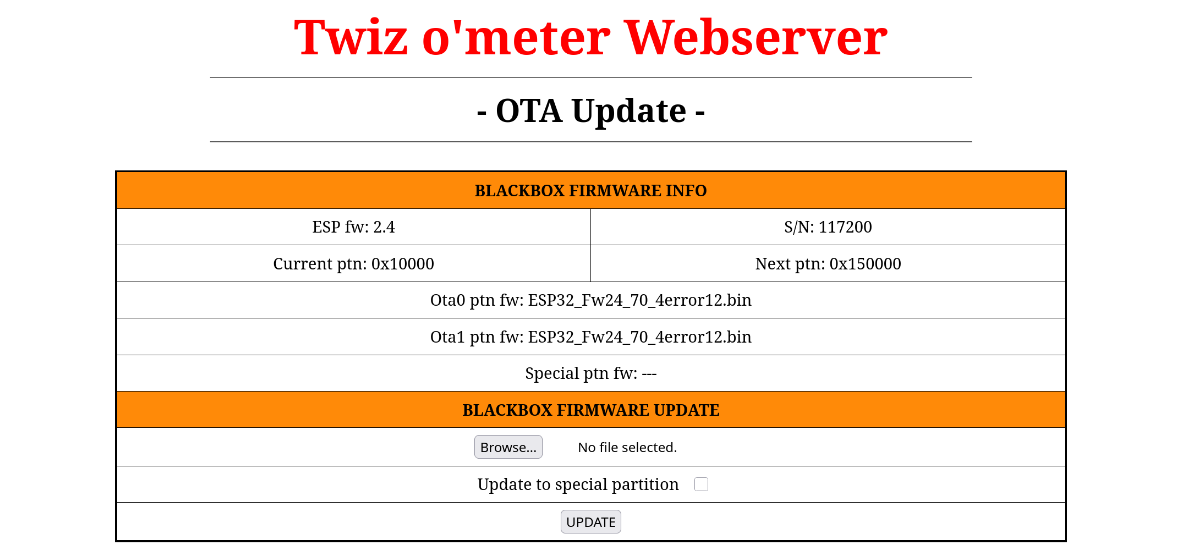
\includegraphics[width=1\textwidth]{figures/ota_page3.png}
    \caption{Page de mise à jour OTA --- Table de mise à jour et d'informations.}
\end{figure}

Lorsque la barre de progression de la mise à jour atteint 100\%, l'écran LCD du ToM+ devient noir et
c'est le signe concluant que ToM+ redémarre, en chargeant le logiciel \textit{Twizy-cfg}.
Maintenant, vous devez vous connecter au point d'accès \textbf{“Twizy-cfg”} sur votre appareil pour accéder
à son serveur web et, si cela vous est demandé, accepter de maintenir la connexion active même si
elle ne fournit pas d'accès Internet.

Le \textbf{mot de passe} est le mot de passe ToM+ par défaut, c'est-à-dire le mot “pass” suivi du
numéro de série de votre appareil (par ex. \textit{pass129777}). Le numéro de série se trouve sur la
page des paramètres comme expliqué à la Figure~\ref{fig:settings_page}.\\

Maintenant, ouvrez un navigateur web et tapez \textbf{192.168.4.1/webserial} pour naviguer vers
l'interface du serveur web, où vous pouvez envoyer des commandes de réglage. Le terminal de commande ressemble
à celui montré sur l'image ici. Comme déjà dit, le réglage n'est pas une fonctionnalité officielle de ToM+
et \textit{Twizy-cfg} n'a pas été écrit par moi, veuillez donc vous référer au \href{https://www.twizy-forum.de/projekte-twizy/83451-twizy-cfg-sevcon-shell-fuer-arduino?start=0}{sujet Twizy-cfg}
ou à son \href{https://github.com/dexterbg/Twizy-Cfg}{dépôt Github} pour connaître les
commandes et configurations de réglage.\\

\begin{figure}[H]
    \centering
    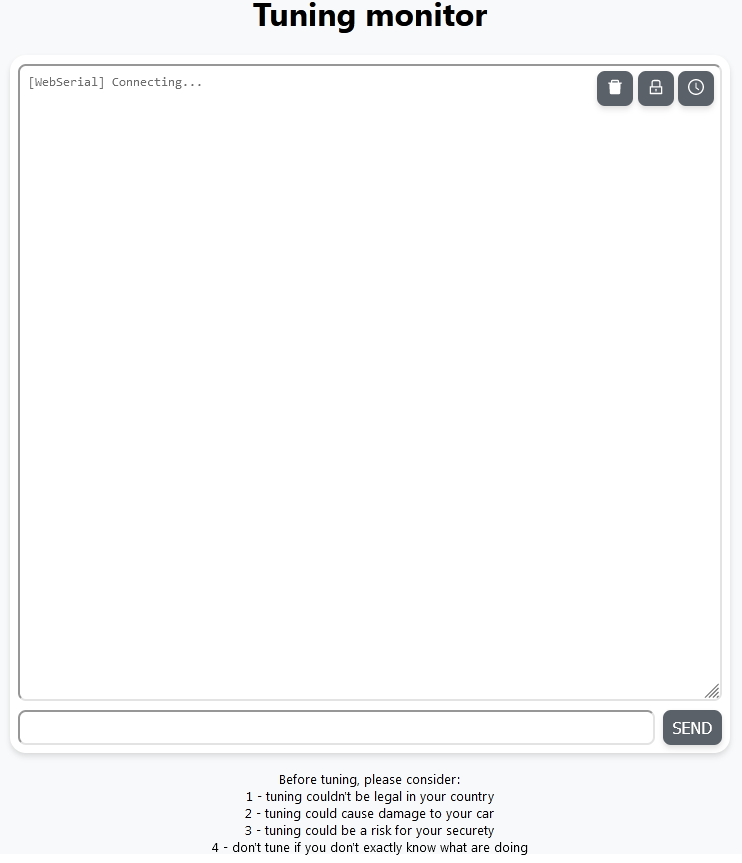
\includegraphics[width=0.7\textwidth]{figures/TuningMonitor.PNG}
    \caption{Moniteur de réglage pour exécuter les commandes de configuration.}
\end{figure}

Tant que vous utilisez Twizy-cfg, le micrologiciel ToM+ ne sera pas chargé et l'écran ne s'allumera
donc pas. Lorsque vous souhaitez revenir au micrologiciel officiel ToM+, il vous suffira de taper
dans le moniteur de réglage cette commande explicite : \textbf{reboot}.\\

Et voilà, ToM+ redémarre sur l'autre partition et revient à son comportement normal,
et la configuration de réglage persistera dans votre Twizy. La prochaine fois
que vous aurez besoin du shell Twizy-cfg, allez simplement sur la page \textbf{“OTA Update and Prefs”}
du serveur web ToM+ et sélectionnez l'option \textit{“REBOOT FROM SPECIAL PARTITION”}
dans le tableau présenté dans l'image suivante. Pas besoin de téléverser à nouveau le fichier \textit{“.bin”}.

\begin{figure}[H]
    \centering
    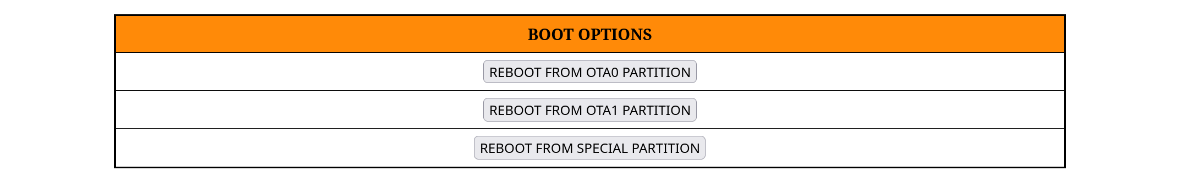
\includegraphics[width=1\textwidth]{figures/ota_boot.png}
    \caption{Page de mise à jour OTA --- Tableau des options de démarrage.}
\end{figure}


\chapter{Contrôle de l'interrupteur WiFi Tasmota}
\label{apx:tasmota}

\section{Que sont les interrupteurs/prises WiFi ?}

Dans cet appendice, j'expliquerai comment vous pouvez configurer votre ToM+ pour interagir avec un interrupteur
AC WiFi / une prise AC, ou tout autre appareil exécutant un \textbf{micrologiciel Tasmota}.

Il s'agit essentiellement de \textit{modules relais} qui peuvent être contrôlés à distance via une connexion sans fil.
Vous pouvez facilement trouver ce genre d'appareils sur de nombreux sites d'e-commerce (comme Amazon),
pour quelques dizaines d'euros.\\

Ils existent sous plusieurs formats, mais ils apparaissent fréquemment sous les deux formes montrées dans l'image.
La seconde est plus compacte et conviviale, tandis que la première nécessite des connexions
par câble pour fonctionner avec vos équipements électriques.

\begin{figure}[ht]
    \centering
    \begin{subfigure}[t]{0.48\textwidth}
        \centering
        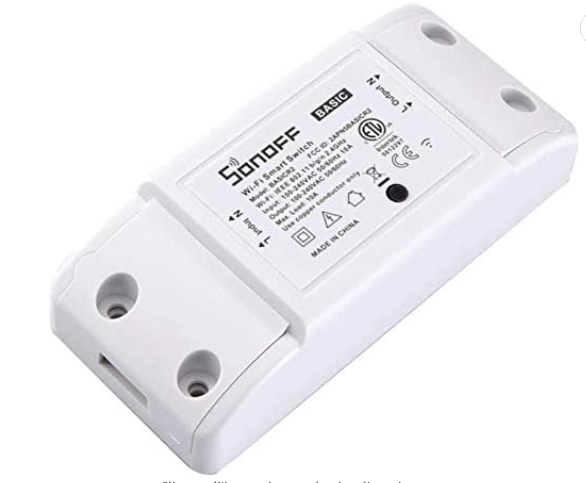
\includegraphics[width=\linewidth]{figures/Sonoff.PNG}
        \caption{Interrupteur intelligent WiFi Sonoff.}
    \end{subfigure}
    \hfill
    \begin{subfigure}[t]{0.48\textwidth}
        \centering
        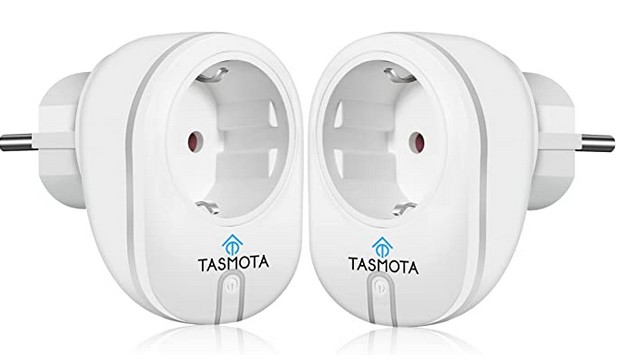
\includegraphics[width=\linewidth]{figures/TasmotaPlug.PNG}
        \caption{Prise intelligente WiFi Tasmota.}
    \end{subfigure}
\end{figure}

\textit{Mais pourquoi est-ce utile ?} Il existe de nombreuses raisons pour lesquelles vous pourriez avoir besoin de connecter ToM+ à ces appareils.
Par exemple : vous souhaitez arrêter la charge de la batterie de traction si le chargeur surchauffe et
reprendre la charge lorsque la température diminue ; ou peut-être souhaitez-vous \textbf{arrêter la charge}
lorsqu'un SOC souhaité est atteint.

Ou encore, comme je l'ai fait dans cet appendice à des fins expérimentales, pour allumer une lampe dans ma
chambre lorsque la Twizy (garée dans le garage) a presque terminé sa charge.
En résumé, il existe de nombreuses idées utiles où un interrupteur/prise WiFi combiné à
ToM+ peut aider à créer de superbes projets.


\section{Prérequis avant de commencer}

Pour atteindre cet objectif, vous aurez besoin d'une boîte noire exécutant une version de micrologiciel \textbf{1.4}
ou supérieure. Il s'agit d'une exigence cruciale, car ce processus nécessite des
fonctionnalités introduites dans la version mentionnée. Consultez la Section~\ref{sec:settings_page}
pour vérifier la version du micrologiciel de votre ESP et la Section~\ref{sec:web_ota_update} pour mettre à
jour votre micrologiciel via OTA si nécessaire.

De plus, vous devrez avoir \textbf{configuré le WiFi et MQTT} pour faire fonctionner
l'ensemble du système. Si ce n'est pas le cas, veuillez vous référer à la Section~\ref{sec:wifi_settings} pour configurer le WiFi et à la
Section~\ref{sec:mqtt_connection} pour la configuration MQTT. Ils doivent tous deux être
activés et connectés pour accomplir cette tâche.\\

Ensuite, vous aurez évidemment besoin d'un interrupteur ou d'une prise sans fil, selon vos besoins, et
il doit exécuter un \textbf{micrologiciel Tasmota} (\textit{version 7} ou supérieure).

Gardez à l'esprit que les appareils de type \textit{“Sonoff”} sortent d'usine avec un micrologiciel
propriétaire qui ne prend pas en charge nativement le protocole MQTT.\\

Afin de les utiliser, comme je l'ai fait dans cet appendice, vous devez les mettre à niveau vers le micrologiciel Tasmota.
Le web regorge de guides sur l'installation du micrologiciel Tasmota, recherchez donc celui qui
convient à votre appareil et suivez-le.
Pour les utilisateurs qui ne souhaitent pas effectuer la procédure de mise à jour du micrologiciel, je suggère personnellement
d'acheter un appareil fonctionnant déjà sous le micrologiciel Tasmota.


\section{Configuration MQTT de Tasmota}

Naviguez vers l'interface \textbf{Tasmota WebUI} et vous obtiendrez une page d'accueil similaire à celle
présentée ci-dessous. À tout moment, en cas de doute, veuillez consulter la \href{https://tasmota.github.io/docs/}{documentation officielle}.

\begin{figure}[H]
    \centering
    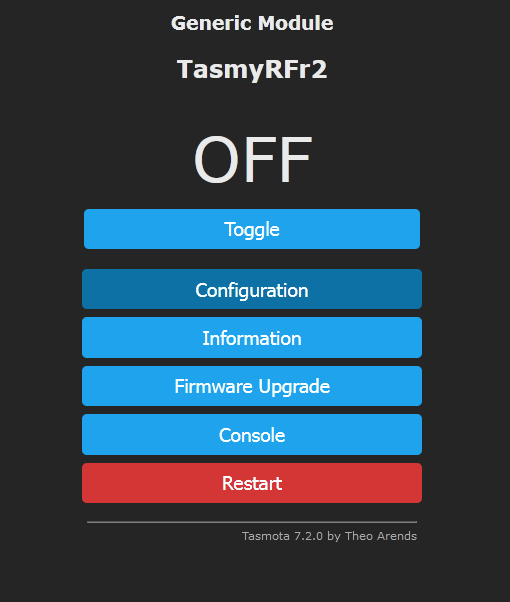
\includegraphics[width=0.45\textwidth]{figures/Mqtt1.PNG}
    \caption{Tasmota webUI --- Page d'accueil.}
\end{figure}

Tout d'abord, appuyez sur le bouton \textbf{“Configuration”} qui vous mènera à la page montrée
dans la première image ci-dessous.
Ensuite, configurez la \textit{connexion WiFi}, en entrant vos paramètres (SSID et mot de passe) dans la
page \textbf{“Configure WiFi”} de Tasmota. Ensuite, suivez les instructions pour configurer
les \textit{paramètres MQTT}, en accédant à la page webUI \textbf{“Configure MQTT”}.\\

\clearpage

\begin{figure}[ht]
    
    \begin{subfigure}[t]{0.4\textwidth}
        \centering
        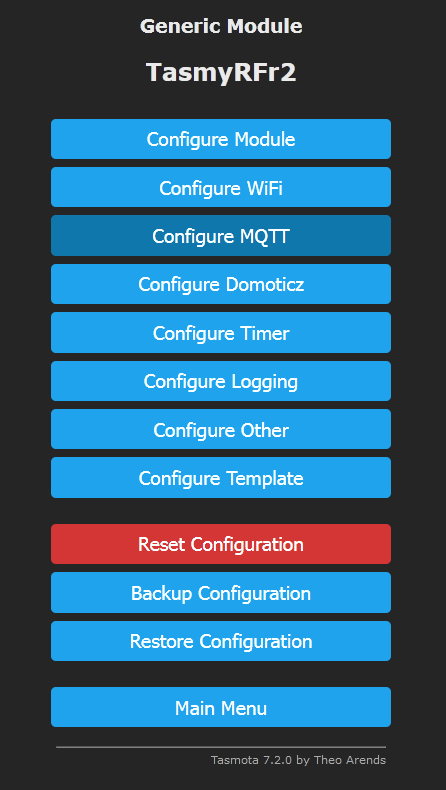
\includegraphics[width=\linewidth]{figures/Mqtt2.PNG}
        \caption{Page de configuration.}
    \end{subfigure}
    \hfill
    \begin{subfigure}[t]{0.48\textwidth}
        \centering
        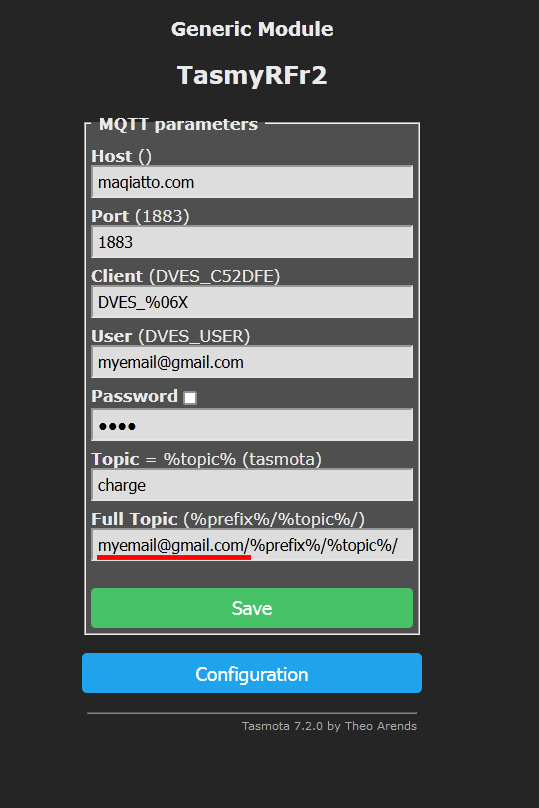
\includegraphics[width=\linewidth]{figures/Mqtt4.PNG}
        \caption{Page de configuration MQTT.}
    \end{subfigure}
\end{figure}

Entrez maintenant l'adresse de votre broker, votre ID utilisateur, votre mot de passe et le numéro de port. Ils doivent être les mêmes
que ceux définis sur ToM+ ! Vous pouvez consulter l'explication de chaque champ dans la Section~\ref{sec:mqtt_connection}.\\

Les paramètres les plus difficiles à comprendre sont \textbf{“Topic”} et \textbf{“Full Topic”}.
Ceux-ci ne doivent pas être identiques aux topics MQTT de ToM+, car ils sont spécifiques à l'appareil que vous utilisez.
Si vous mettez les mêmes topics \textit{TOMin} et \textit{TOMout}, les communications risquent de se
perturber mutuellement.\\

Dans le premier champ, entrez ce que vous voulez. Je suggère quelque chose qui rappelle la
fonction de votre appareil. Mais veuillez utiliser une chaîne courte (5/6 caractères suffisent), car ce
champ sera une partie minimale de la chaîne du topic complet et ToM+ a une limite de 50 caractères
pour le champ \textbf{“Auxilliary MQTT command”} (discuté dans la Section~\ref{sec:web_alarm_triggers}).

Dans le second champ, il est important de distinguer deux options, selon le
broker que vous utilisez. Si vous avez votre propre broker (c'est-à-dire \textit{pas Maqiatto}),
laissez la chaîne par défaut \textbf{\%prefix\%/\%topic\%/}.\\

Si vous utilisez plutôt Maqiatto, configuré selon la Section~\ref{sec:free_broker} ou 
tout autre broker qui ajoute \textit{votre e-mail comme préfixe} du nom de topic, alors
modifiez le champ \textbf{“Full Topic”} en conséquence. \linebreak Les champs seront ceux présentés 
dans la deuxième image ci-dessus, ce qui donne \linebreak \textbf{myemail@gmail.com/\%prefix\%/\%topic\%/},
en ajoutant votre userID (e-mail) comme préfixe.

Enfin, appuyez sur le bouton vert \textbf{“Save”} et attendez que l'appareil redémarre.\\

\textbf{RAPPEL !} Si vous utilisez le broker Maqiatto, vous devrez peut-être ajouter le nouveau topic
à votre compte comme expliqué à la Figure~\ref{sec:free_broker_add_topics}.

Dans ce cas, vous devrez ajouter \textbf{cmnd/<votre\textunderscore~nom\textunderscore~de\textunderscore~topic\textunderscore~Tasmota>/Power} comme nouveau nom de topic,
qui deviendra \textit{cmnd/charge/Power} si vous avez suivi l'image.


\section{Configuration Tasmota sur ToM+}

Ouvrez le serveur web ToM+ comme expliqué dans la Section~\ref{sec:web_server_access} et allez sur la
page \textbf{“Alarm triggers”}. Maintenant, ajoutez une nouvelle alarme à la liste en fonction de
l'élément qui contrôlera votre appareil Tasmota, comme expliqué dans la Section~\ref{sec:web_alarm_triggers}.

Dans mon cas, j'ai choisi l'élément \textbf{“Battery SOC”}, qui déclenchera l'alarme lorsque sa
valeur sera \textit{égale à 97\%}, pour notifier que la charge est presque terminée.

\begin{figure}[H]
    \centering
    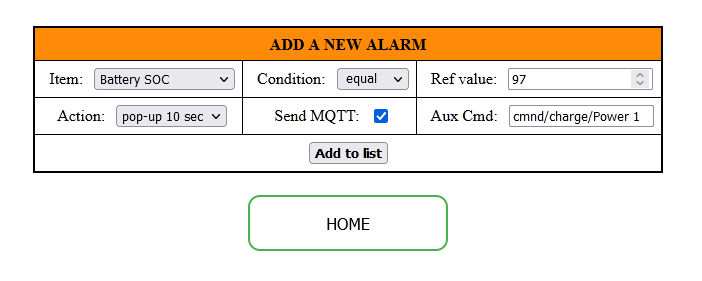
\includegraphics[width=0.7\textwidth]{figures/Tom01.PNG}
    \caption{Ajout du déclencheur Tasmota sur ToM+.}
\end{figure}

Comme vous pouvez le remarquer, la partie la plus importante est de configurer correctement le champ \textbf{“Aux Cmd”},
car il contient la commande MQTT de contrôle que ToM+ enverra à
l'appareil Tasmota.

Si vous avez votre propre broker MQTT (c'est-à-dire \textit{pas Maqiatto}), la \textbf{Aux Cmd} aura cette syntaxe :
\begin{itemize}
    \item \textit{cmnd/<votre\textunderscore~nom\textunderscore~de\textunderscore~topic\textunderscore~Tasmota>/Power 1} si vous souhaitez allumer l'appareil.
    \item \textit{cmnd/<votre\textunderscore~nom\textunderscore~de\textunderscore~topic\textunderscore~Tasmota>/Power 0} si vous souhaitez l'éteindre.
\end{itemize}
À nouveau, dans notre exemple, la commande devient \textbf{cmnd/charge/Power 1} pour allumer la lampe.\\

Sinon, si vous utilisez le broker Maqiatto ou un autre qui utilise votre userID (e-mail)
comme préfixe dans le nom des topics, la syntaxe de la \textbf{Aux Cmd} ressemblera à ceci :
\begin{itemize}
    \item \textit{myemail@gmail.com/cmnd/<votre\textunderscore~nom\textunderscore~de\textunderscore~topic\textunderscore~Tasmota>/Power 1} pour l'allumer.
    \item \textit{myemail@gmail.com/cmnd/<votre\textunderscore~nom\textunderscore~de\textunderscore~topic\textunderscore~Tasmota>/Power 0} pour l'éteindre.
\end{itemize}
Dans notre cas, la commande devient \textbf{myemail@gmail.com/cmnd/charge/Power 1}.\\

Si vous souhaitez arrêter la charge puis la redémarrer lorsque des conditions spécifiques sont remplies, vous
devez ajouter deux alarmes, une pour chaque condition d'allumage/extinction (Power ON/OFF), en utilisant la syntaxe expliquée en conséquence.\\

Veuillez noter que si vous avez un appareil avec plusieurs relais, vous devrez 
modifier la syntaxe ci-dessus en spécifiant quel relais vous souhaitez contrôler : en utilisant \textbf{“Power1”}
pour le premier relais, \textbf{“Power2”} pour le second et ainsi de suite. Cela devient :
\begin{itemize} 
    \item \textit{cmnd/<votre\textunderscore~nom\textunderscore~de\textunderscore~topic\textunderscore~Tasmota>/Power1 1} pour allumer le premier relais.
    \item \textit{cmnd/<votre\textunderscore~nom\textunderscore~de\textunderscore~topic\textunderscore~Tasmota>/Power1 0} pour l'éteindre.
\end{itemize}
La même distinction de syntaxe concernant Maqiatto et les brokers possédés s'applique également ici.

\section{Problèmes courants et solutions}

Certains micrologiciels Tasmota n'aiment pas le format de topic \textit{Maqiatto}, donc si vous souhaitez 
piloter un appareil Tasmota avec ToM+, vous devez utiliser un autre broker MQTT.
Après quelques tests, j'ai remarqué que vous pouvez utiliser avec succès \href{https://dealgate.ru/}{mqtt.dealgate.ru},
gratuit et plus riche en fonctionnalités. 

L'inconvénient est que vous devez faire face à quelques traductions en russe pour créer le compte.
Mais rien qu'un traducteur en ligne ne puisse résoudre.
